% fig06_pair_threshold.tex — pair-production: available CM energy vs lab beam energy.
% Compiled by the paper Makefile via `make figures` (pdflatex on the snippet).
%
% Data provenance (NO fabrication; commons @D g3) — Appendix A (app:production):
%   Fixed-target p+p: total CM energy sqrt(s) = sqrt(2 m_p c^2 (T_beam + 2 m_p c^2)),
%     with m_p c^2 = 938.272 MeV. The pair-production channel p+p->p+p+pbar+p
%     opens when sqrt(s) >= 4 m_p c^2 (four final nucleons at rest in CM).
%   Registered verify-atom anchor (vertical line + marker):
%     E_beam,th = 7 m_p c^2 = 6567.9 MeV (pair_threshold_total, PR #1014),
%     where sqrt(s) = 4 m_p c^2 = 3753.1 MeV exactly. The integer factor 7 is
%     the BLUE-MAX atom pair_threshold_total_factor=7 (PR #1094).
%   No off-anchor experimental cross-section points are invented; only the exact
%     kinematic curve and the single registered threshold anchor are plotted.
%
% Manual single-shot compile (debug):
%   pdflatex -interaction=nonstopmode -halt-on-error fig06_pair_threshold.tex
\documentclass[border=4pt]{standalone}
\usepackage{tikz}
\usepackage{pgfplots}
\pgfplotsset{compat=1.18}
\begin{document}
% sqrt(s) = sqrt(2*938.272*(x + 2*938.272))  [MeV], x = beam kinetic T_beam (MeV)
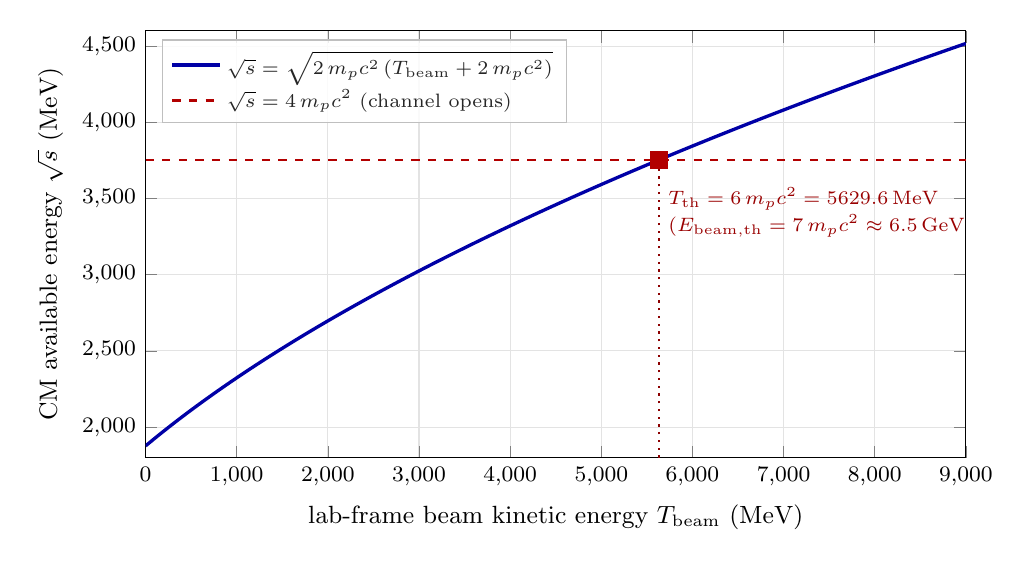
\begin{tikzpicture}
\begin{axis}[
  width=12cm, height=7cm,
  xlabel={lab-frame beam kinetic energy $T_{\mathrm{beam}}$ (MeV)},
  ylabel={CM available energy $\sqrt{s}$ (MeV)},
  xmin=0, xmax=9000,
  ymin=1800, ymax=4600,
  tick label style={font=\footnotesize},
  label style={font=\small},
  ymajorgrids, xmajorgrids, grid style={gray!22},
  legend style={font=\scriptsize, at={(0.02,0.98)}, anchor=north west,
    fill=white, fill opacity=0.85, draw=gray!50},
  legend cell align=left,
]
% --- CM energy curve sqrt(s)(T_beam) ---
\addplot[blue!65!black, very thick, smooth, domain=0:9000, samples=120] {
  sqrt(2*938.272*(x + 2*938.272))
};
\addlegendentry{$\sqrt{s}=\sqrt{2\,m_pc^2\,(T_{\mathrm{beam}}+2\,m_pc^2)}$}
% --- pair-production threshold line sqrt(s) = 4 m_p c^2 = 3753.088 MeV ---
\addplot[red!70!black, dashed, thick, domain=0:9000, samples=2] {3753.088};
\addlegendentry{$\sqrt{s}=4\,m_pc^2$ (channel opens)}
% --- registered verify-atom anchor: T_beam = 6 m_p c^2 (kinetic), beam total = 7 m_p c^2 ---
\addplot[only marks, mark=square*, mark size=3pt, red!70!black] coordinates {
  (5629.63, 3753.088)
};
\node[font=\scriptsize, anchor=west, text=red!60!black] at (axis cs:5629.63,3500) {%
  $T_{\mathrm{th}}=6\,m_pc^2=5629.6$\,MeV};
\node[font=\scriptsize, anchor=west, text=red!60!black] at (axis cs:5629.63,3320) {%
  ($E_{\mathrm{beam,th}}=7\,m_pc^2\approx6.5$\,GeV)};
% threshold vertical guide
\draw[red!55!black, dotted, thick] (axis cs:5629.63,1800) -- (axis cs:5629.63,3753.088);
\end{axis}
\end{tikzpicture}
\end{document}
